%\documentclass[aps,prl,twocolumn,preprintnumbers,groupedaddress]{revtex4}
\documentclass[aps,prl,preprint,preprintnumbers,groupedaddress]{revtex4}

\usepackage{graphicx}
\usepackage{color}

\newcommand{\eps}{\varepsilon}
\newcommand{\vecr}{\vec{r}}
\newcommand{\vecu}{\vec{u}}
\newcommand{\vecJ}{\vec{J}}
\newcommand{\vecP}{\vec{P}}
\newcommand{\vecE}{\vec{E}}
\newcommand{\vecB}{\vec{B}}
\newcommand{\tensT}{\mathbf{T}}
\newcommand{\tensP}{\mathbf{\Pi}}
\newcommand{\tensS}{\mathbf{\Xi}}
\newcommand{\EN}{\mathcal{E}}
\newcommand{\op}{\mathcal{L}}

\newcommand{\Expect}[1]{\left< #1 \right>}
\newcommand{\Deriv}[2]{d_{#2}#1}
\newcommand{\PDeriv}[2]{\partial_{#2}#1}

\newcommand{\DotP}[2]{#1 \cdot #2}
\newcommand{\CrossP}[2]{#1 \times #2}

\newcommand{\Grad}[1]{\nabla #1}
\newcommand{\Div}[1]{\nabla \cdot #1}
\newcommand{\Curl}[1]{\nabla \times #1}

\newcommand{\Gradu}[1]{\nabla_{\vecu} #1}
\newcommand{\Divu}[1]{\nabla_{\vecu} \cdot #1}
\newcommand{\Curlu}[1]{\nabla_{\vecu} \times #1}

\newcommand{\eq}[1]{(\ref{eq:#1})}
\newcommand{\tbl}[1]{Table \ref{tbl:#1}}
\newcommand{\fig}[1]{Figure \ref{fig:#1}}

\begin{document}

\preprint{LA-UR-07-7527}

\title{Ultra high performance 3d electromagnetic relativistic kinetic plasma simulation}

\author{K.~J.~Bowers}
\email{kevin.j.bowers@gmail.com}
\altaffiliation[Guest Scientist.  Presently at ]{
  D.~E.~Shaw Research LLC,
  120 W 45th St, 39th Fl,
  New York, NY 10036
}
\author{B.~J.~Albright}
\author{L.~Yin}
\author{B.~Bergen}
\author{T.~J.~T.~Kwan}
\affiliation{
  Plasma Theory and Applications (X-1-PTA),
  Los Alamos National Laboratory,
  MS F699, PO Box 1663,
  Los Alamos, NM, 87545
}

\date{\today}

\begin{abstract}
The algorithms, implementation details and applications of VPIC, a
state-of-the-art first principles 3d electromagnetic relativistic
kinetic particle-in-cell code, are discussed.  Unlike most codes, VPIC
is designed to minimize data motion, as, due to physical limitations
(including the speed of light!), moving data between and even within
modern microprocessors is more time consuming than performing
computations.  As a result, VPIC has achieved unprecedented levels of
performance.  For example, VPIC can perform $\sim 0.17$ billion cold
particles pushed and charge conserving accumulated per second per
processor on IBM's Cell microprocessor---equivalent to sustaining Los
Alamos's planned Roadrunner supercomputer at $\sim 0.56$ petaflop
(quadrillion floating point operations per second).  VPIC has enabled
previously intractable simulations in numerous areas of plasma
physics, including magnetic reconnection and laser plasma
interactions; next generation supercomputers like Roadrunner will
enable further advances.
\end{abstract}

\maketitle

\section{Introduction}

In many settings in plasma physics, first principles particle-in-cell
(PIC) simulation \cite{Birdsall_Langdon_1985,Hockney_Eastwood_1988} is
the only viable tool for understanding the physics.  By their nature,
large scale explicit PIC simulations require large computing
resources.  Traditional programming methodologies, evolved from
experience on large vector single instruction multiple data (SIMD)
machines, no longer utilize these resources efficiently; minimizing
data motion is now paramount.  This work gives an overview of the 3d
relativistic electromagnetic PIC code VPIC.  VPIC uses state of the
art algorithms and optimizes data flows used by these algorithms
for modern supercomputers.  Several example simulations enabled by
VPIC's unprecented performance are shown.  The techniques used in
VPIC, outlined below, can be used in many other simulations codes.

\section{VPIC Algorithms}

\subsection{PIC Overview}

VPIC integrates the relativistic Maxwell-Boltzmann equations in a
linear background medium
\begin{eqnarray}
\PDeriv{f_s}{t} &+& 
\DotP{c\gamma^{-1}\vecu}{\Grad{f_s}} +
\DotP{\frac{q_s}{m_s c} \left( \vecE + \CrossP{c\gamma^{-1}\vecu}{\vecB} \right)}{\Gradu{f_s}} \nonumber\\
&=& \left(\PDeriv{f_s}{t}\right)_{coll}
\label{eq:Boltzmann}\\
\PDeriv{\vecB}{t} &=& -\Curl{\vecE}
\label{eq:Faraday}\\
\PDeriv{\vecE}{t} &=&
\eps^{-1}\Curl{\mu^{-1}\vecB} - \eps^{-1}\vecJ - \eps^{-1}\sigma\vecE
\label{eq:Ampere}
.
\end{eqnarray}
Above, $f_s\left(\vecr,\vecu,t\right)$ is the smooth part of the
instantaneous phase-space distribution of a species $s$ with particle
charge $q_s$ and mass $m_s$.  $c$ is the speed of light in vacuum,
$\vecu$ is the normalized momentum and $\gamma\left(\vecu\right) =
\sqrt{1 + u^2}$ is the relativistic factor.
$\vecE\left(\vecr,t\right)$ and $\vecB\left(\vecr,t\right)$ are the
electric and magnetic field and $\vecJ\left(\vecr,t\right) =
\sum_s \int d\vecu q_s c\gamma^{-1}\vecu f_s$ is the current
density.  $\eps\left(\vecr\right)$, $\mu\left(\vecr\right)$ and
$\sigma\left(\vecr\right)$ are the background medium diagonal
permittivity, permeability and conductivity tensors.
$\left(\PDeriv{f_s}{t}\right)_{coll}$ represents discrete
particle effects (e.g. short range Coulomb collisions, excitation and
ionization).

Since a direct discretization of $f_s$ is prohibitive, PIC simulations
sample it with a collection of computational particles---each
computational particle typically represents many physical particles.
\eq{Boltzmann} is replaced by the computational particle
equation of motions
\begin{eqnarray}
\Deriv{r_{s,n}}{t} &=& c \gamma_{s,n}^{-1} \vecu_{s,n} \label{eq:Position}\\
\Deriv{u_{s,n}}{t} &=& \frac{q_s}{m_s c} \left[
\vecE\left(\vecr_{s,n},t\right) +
\CrossP{c\gamma_{s,n}^{-1}\vecu_{s,n}}{\vecB\left(\vecr_{s,n},t\right)}
\right] \label{eq:Momentum}
\end{eqnarray}
$f_s$ for the computational particles obeys \eq{Boltzmann} outside of
discrete particle collisional effects.  A smooth $\vecJ$ is computed
from the particle motion for use in \eq{Faraday}-\eq{Ampere}.  Because
$\vecJ$ is smooth, $\vecE$, $\vecB$ and $\vecJ$ can be sampled on a
mesh and interpolated between the mesh and particles.

PIC simulations of these equations can be distinguished by the time
stepping, field discretization, interpolation and collision methods.
VPIC uses state-of-the-art techniques, many of which are in use in
other codes
\cite{Kwan_Snell_1985,Verboncoeur_et_al_1995,Eastwood_et_al_1995,Jones_et_al_1996,Blahovec_et_al_2000,Nieter_Cary_2004}.
The methods are summarized below for completeness; more in-depth
analysis of PIC simulation can be found in
\cite{Birdsall_Langdon_1985,Hockney_Eastwood_1988}.  For the sake of
brevity, collisional methods will not be discussed in this paper.

\subsection{Time and space discretization}

The formal solution to $\Deriv{X}{t} = \op X$ for a well-behaved
operator $\op$ on $X\left(t\right)$ is $X\left(t+\delta_t\right) =
e^{\delta_t\op} X\left(t\right)$.  If $\op$ can be split into the sum
of $N$ well-behaved operators, $\op = \sum_i \op_i$, the operator
exponential can be approximated to second order in $\delta_t$ by
$e^{\delta_t\op} \approx e^{\delta_t\op_1/2} e^{\delta_t\op_2/2} ...
e^{\delta_t\op_{N-1}/2} e^{\delta_t\op_N} e^{\delta_t\op_{N-1}/2} ...
e^{\delta_t\op_2/2} e^{\delta_t\op_1/2}$
\cite{McLachlan_Quispel_2002}.  One splitting for
\eq{Faraday}-\eq{Momentum} is
\begin{eqnarray}
e^{\delta_t\op}&\approx& e^{\delta_t\op_{ub}/2} e^{\delta_t\op_{ue}/2}
e^{\delta_t\op_r/2} \nonumber\\
& & e^{\delta_t\op_B/2}e^{\delta_t\op_E} e^{\delta_t\op_B/2} \nonumber\\
& & e^{\delta_t\op_r/2} e^{\delta_t\op_{ue}/2} e^{\delta_t\op_{ub}/2}
,
\label{eq:Operator_Split}
\end{eqnarray}
where
\begin{eqnarray}
\op_B    &:& \PDeriv{\vecB}{t} = -\Curl{\vecE} \\
\op_E    &:& \PDeriv{\vecE}{t} =
\eps^{-1}\Curl{\mu^{-1}\vecB} - \eps^{-1}\vecJ - \eps^{-1}\sigma\vecE \\
\op_{r}  &:& \Deriv{\vecr_{s,n}}{t} = c\gamma_{s,n}^{-1}\vecu_{s,n} \\
\op_{ue} &:& \Deriv{\vecu_{s,n}}{t} =
\frac{q_s}{m_s c} \vecE\left(\vecr_{s,n},t\right) \\
\op_{ub} &:& \Deriv{\vecu_{s,n}}{t} = \CrossP{\vecu_{s,n}}
{\frac{q_s}{m_s\gamma_{s,n}}\vecB\left(\vecr_{s,n},t\right)}
.
\end{eqnarray}

Consider the repeated application of \eq{Operator_Split}.  Grouping
the updates to $\vecE$ and $\vecB$ separately and noting the effect of
$e^{\delta_t\op_r/2}$ is independent of $\vecE$ and $\vecB$ yields a
time step that can be implemented efficiently:
\begin{eqnarray}
\text{Particle advance} &:& e^{\delta_t\op_r/2} I_J e^{\delta_t\op_r/2} \nonumber\\
& & e^{\delta_t\op_{ue}/2} e^{\delta_t\op_{ub}} e^{\delta_t\op_{ue}/2}
\label{eq:Particle_advance}\\
\text{Field advance}    &:& e^{\delta_t\op_B/2} e^{\delta_t\op_E} e^{\delta_t\op_B/2} \label{eq:Field_advance}
\end{eqnarray}
$I_J$ indicates that $\vecJ$ is computed for \eq{Field_advance} but
the state is unchanged.  Thus, \eq{Particle_advance} and
\eq{Field_advance} use a mixture of velocity Verlet and leapfrog to
advance $\vecu_{s,n}$ from $t-\delta_t/2$ to $t+\delta/2$ and
$\vecr_{s,n}$, $\vecE$ and $\vecB$ from $t$ to $t+\delta_t$.
% FIXME: EXPLAIN THE GOOD CHI OF A TROTTER EXPANSION HERE?

The simulation domain is divided into a regular mesh of identical
rectangular cells with potentially irregular but cell aligned
boundaries.  $\vecE$ and $\vecB$ are staggered; $E_x$ is sampled at
the middle of $x$-directed cell edges, $B_x$ is sampled at the middle
of $yz$-oriented cell faces and similarly for the $y$ and $z$
components.  $\vecJ$ is sampled the same as $\vecE$.  A variety of
particle and field boundary conditions are supported on the domain
boundaries including particle absorbing, particle reflecting, particle
refluxing, perfect electric conductor, perfect magnetic conductor,
field emitting and field absorbing (first order Higdon
\cite{Higdon_1986}).

\subsection{Particle advance}

In exact arithmetic, $\op_r$ is trivial to apply exactly:
\begin{equation}
e^{\delta_t\op_r} : \vecr_{s,n} \leftarrow \vecr_{s,n} +
\delta_t c\gamma_{s,n}^{-1}\vecu_{s,n}
.
\end{equation}
$\op_{ue}$ is similarly trivial:
\begin{equation}
e^{\delta_t\op_{ue}} : \vecu_{s,n} \leftarrow \vecu_{s,n} +
\frac{q_s\delta_t}{m_s c} \vecE\left(\vecr_{s,n},t\right)
.
\end{equation}
$\op_{ub}$ is more involved but can also be done exactly:
\begin{eqnarray}
e^{\delta_t\op_{ub}} : \vecu_{s,n} &\leftarrow& \text{Rotate } \vecu_{s,n} \text{ around axis } \vecB\left(\vecr_{s,n},t\right) \nonumber\\
& &\text{ by } \frac{q_s\delta_t}{m_s\gamma_{s,n}}\left|\vecB\left(\vecr_{s,n},t\right)\right|
\text{ radians }
\end{eqnarray}
(Note that because magnitude of a vector is invariant under rotation,
$\gamma_{s,n}$ is unchanged and this operator conserves energy.)  This
can be implemented efficiently by a Boris push \cite{Boris_1970}.
Unfortunately, if done exactly as given above, cyclotron motion above
the simulation Nyquist frequency will be aliased.  To avoid this, VPIC
uses a 6th order rotation angle approximation that is also more
efficient to compute.  The numerical cyclotron frequency is nearly
exact for physical cyclotron frequencies below the Nyquist frequency
and asymptotes to the Nyquist frequency otherwise.  The resulting
update still conserves energy and will not non-physically couple high
frequency cyclotron motion to low frequency phenomena.  A similar
method is used in \cite{Blahovec_et_al_2000}.

VPIC uses an energy conserving interpolation scheme for the particle
fields like that in \cite{Eastwood_et_al_1995}.  For example, $E_x$ is
bilinearly interpolated from the four $E_x$ edge samples and $B_x$ is
linearly interpolated from two $B_x$ face samples of the cell
containing a particle.  While this scheme does not yield as smooth a
field interpolation as a momentum conserving trilinear interpolation,
this interpolation is consistent with a finite element time domain
treatment of \eq{Faraday}-\eq{Momentum} for this discretization
\cite{Eastwood_et_al_1995} and is easier to implement in simulations
with irregular boundary conditions as no resampling of field
components is required.

VPIC uses the charge conserving method of Villasenor and Buneman
\cite{Villasenor_Buneman_1992} to compute $\vecJ$ for the
field advance.  A particle makes a $\vecJ$ contribution in each cell
it passes through during a time step.  In exact arithmetic, the
resulting $\vecJ$ satisfies the discretized charge conservation
equation implicit in the field advance described below for a trilinear
$\rho$ accumulation.  Though this is often considered prohibitively
expensive, this eliminates issues that can arise from the build up of
Gauss' law violations.  Further, determining all the cells a particle
passed through provides efficient and robust particle boundary
interaction detection.

\subsection{Field advance}

$\op_B$ is trivial to apply:
\begin{equation}
e^{\delta_t \op_B}: \vecB \leftarrow \vecB - \delta_t \Curl{\vecE}
\label{eq:Discrete_Faraday}
\end{equation}
Likewise, $\op_E$ can be applied exactly:
\begin{eqnarray}
e^{\delta_t \op_E}&:& \vecE \leftarrow e^{-\delta_t \eps^{-1} \sigma} \vecE + \nonumber\\
& & \sigma^{-1}\left( 1 - e^{-\delta_t \eps^{-1} \sigma} \right) \left( \Curl{\mu^{-1}\vecB} - \vecJ \right)
\label{eq:Discrete_Ampere}
\end{eqnarray}
(Note that the second term coefficient asymptotes to
$\delta_t \eps^{-1}$ in the limit $\sigma \rightarrow 0$.)

The needed curls are computed with second order accurate finite
differencing.  For example, the curl component necessary to update a
particular $B_x$ is computed by finite differencing the $E_y$ and
$E_z$ fields on the edges of the face associated with $B_x$.

Charge conservation ($\PDeriv{\rho}{t} = -\Div{\vecJ}$) and
\eq{Ampere} imply Gauss' law ($\Div{\eps\vecE} = \rho$) for all
time provided it holds at some initial time.  Similarly, a charge
conserving $\vecJ$ and \eq{Discrete_Ampere} imply a discretized Gauss'
law.  However, in finite precision, arithmetic error can cause Gauss'
law violations to accumulate over time.  To accommodate, VPIC
periodically applies Marder passes \cite{Marder_1987} tuned
specifically to clean arithmetic error induced violations.  While this
method is local and inexpensive, because $\vecJ$ is charge conserving,
it suffices to use it infrequently to keep Gauss' law satisfied to
near machine precision.

For wavelengths comparable to the cell dimensions, the discretized
speed of light can deviate significantly from $c$.  As a result,
relativistic particle motion can generate non-physical Cherenkov
radiation at these wavelengths.  To combat this, VPIC uses the
transverse current adjustment method discussed in
\cite{Eastwood_et_al_1995}.  Effectively, a transverse current
$\vecJ_T$ that obeys $\vecJ_T = \tau \PDeriv{\left(\vecJ_T -
\Curl{\mu^{-1}\vecB}\right)}{t}$ is included in \eq{Discrete_Ampere}.
This inexpensive local method damps short wavelength radiation modes
on a timescale $\tau$ while leaving the long wavelength radiation
modes virtually unaffected and the charge conservation properties of
\eq{Discrete_Ampere} unchanged.

\subsection{Stability}

Consider a simulation in vacuum.  The field advance reduces to a basic
FDTD algorithm \cite{Yee_1966} and the time step and mesh spacing must
satisfy the Courant condition:
\begin{equation}
\left(\frac{c\delta_t}{\delta_x}\right)^2 +
\left(\frac{c\delta_t}{\delta_y}\right)^2 +
\left(\frac{c\delta_t}{\delta_z}\right)^2 < 1
\end{equation}
Additionally, the particle advance usually requires the time step and
cell dimensions to satisfy:
\begin{eqnarray}
\omega_p \delta_t < 2 \\
\delta_{x,y,z} \approx \lambda_d
\end{eqnarray}
where $\omega_p$ is the peak plasma frequency and $\lambda_d$ is the
plasma Debye length.  Given particles cannot exceed $c$, in practice,
satisfying the Courant condition and the Debye criterion typically
implicitly satisfy the plasma frequency criterion.  Though the time
step is stable for any cyclotron frequency, it is usually desirable to
resolve it to keep dynamics accurate.  Also, sampling $f_s$ typically
requires between tens and thousands of particles per cell depending on
the above parameters and phenomena being studied to avoid non-physical
computational particle collisional effects.

\section{VPIC Implementation}

\subsection{Performance guidelines and optimization regime}

\begin{table}
\begin{tabular}{l l || c | c}
\multicolumn{2}{c||}{Operation} & Time & Rel.~Cost \\
\hline
\hline
Data access      & Internode & 10 $\mu$s & 100,000 \\
(Latency)        & Memory    & 50 ns     & 500     \\
                 & L2 Cache  & 5.0 ns    & 50      \\
                 & L1 Cache  & 1.0 ns    & 10      \\
\hline
Data movement    & Internode & 5.0 ns    & 50      \\
(32-bit)         & Memory    & 0.5 ns    & 5       \\
                 & L2 Cache  & 0.2 ns    & 2       \\
                 & L1 Cache  & 0.1 ns    & 1       \\
\hline
Single precision & FLOP      & 0.1 ns    & 1
\end{tabular}
\caption{\label{tbl:Rules_of_thumb}
VPIC implementation rules of thumb.  Data access estimates the time to
initiate a data transfer between the processor and a level in its
memory hierarchy.  Data movement estimates the time to move the next
32-bits in a transfer.  Internode figures were obtained from
benchmarks of typical high performance cluster interconnects.  The
single precision figure corresponds to a 2.5 GHz processor completing
a 4-vector SIMD instruction every clock.  Other rules of thumb were
similarly extrapolated from various data sheets and benchmarks.
Similar rules of thumb were applied in \cite{Bowers_et_al_2006}.}
\end{table}

Most modern supercomputers consist of a large number of parallel
processing nodes connected by network.  The nodes themselves contain
one or more processors and memory.  Processor performance has improved
more rapidly than memory performance over recent decades.  To
compensate, modern processors use a deep memory hierarchy with faster
(though smaller and more limited) ``cache'' memories located close to
the processor.  Approximate rules of thumb for the cost of various
operations on processing nodes are given in \tbl{Rules_of_thumb}.
Achieving high performance requires minimizing latency, bandwidth and
computation, in roughly that order.  As physical constraints (such as
$c$) are already a noticeable component in many costs, the ratio
between processor and memory performance (particularly latency) should
not be expected to improve significantly in the future.

Fortunately, in most parallel relativistic codes, data needed for
computations on a node are spatially localized to that node or very
nearby; internode latency and bandwidth are naturally optimized and
these codes scale very well on parallel computers.  Accordingly, in
VPIC, local data motion is the dominant concern.  Unfortunately, on
most processors, programmers have no control over cache.  Rather, a
processor heuristically caches data it anticipates will be used.
Given this and \tbl{Rules_of_thumb}, minimizing local data motion
requires grouping data needed to perform critical operations
contiguously and accessing it sequentially when possible.  As
computation and storage are virtually free compared to data motion,
replicating computations and/or data is often worthwhile.

In 3D PIC simulations, there tend to be many particles per cell on
average and more field and particle data per node than can fit in any
cache on that node.  In such a simulation, computation time is heavily
dominated by the particle advance.  VPIC is designed for this regime.
For the sake of brevity, only particle advance implementation
considerations are given and simulations will be assumed to be in this
regime.

\subsection{Single precision}

Single precision implementations can be made to run significantly
faster than their double precision counterparts as most modern
processors provide 4-vector single precision SIMD capabilities and
single precision requires half the data movement as double precision.
For typical time steps, cell dimensions and particles per cell,
discretization error exceeds single precision arithmetic error.  Thus,
single precision should be acceptable for such simulations provided it
does not introduce non-physical artifacts (e.g. large violations of
otherwise conserved quantities during the simulation).  VPIC uses
single precision to help achieve high performance but takes care to
structure operations to minimize its impact; some cases are discussed
below.

Unfortunately, languages like C and FORTRAN are not expressive enough
(e.g. data alignment restrictions) to allow compilers to use 4-vector
SIMD in operations as complex as those in VPIC.  To compensate, VPIC
has a C language extension that allows portable 4-vector SIMD code to
be written and converted automatically to high performance 4-vector
SIMD instructions on a wide variety of platforms.  A similar approach
was used in \cite{Bowers_et_al_2006}.

A full discussion of single precision issues is beyond the scope of
this paper.  For examples of single precision use in applications with
far more demanding precision requirements, see
\cite{Bowers_et_al_2006,Lippert_et_al_2007,Langou_et_al_2006}.

\subsection{Single pass processing and particle data layout}

Since there is more particle data than can fit in any cache, it is
desirable to limit the number of times a particle is touched during a
time step lest performance be limited by moving particle data to and
from memory.  This can be achieved by processing the majority of the
particles in a single pass.  This, combined with
\eq{Particle_advance}, yields VPIC's inner loop structure:
\begin{verbatim}
for each particle
  interpolate fields
  update momentum
  update position
  accumulate current
end for
\end{verbatim}

To further minimize the cost of moving particle data, particle data is
stored contiguously, memory aligned and organized for 4-vector SIMD.
A particle looks like:
\begin{verbatim}
struct { float dx, dy, dz; int i;
         float ux, uy, uz; float q; }
\end{verbatim}
As a result, the inner loop streams through particle data once using
large aligned memory transfers under the hood---the ideal memory
access pattern.

\subsection{Field interpolation and particle sorting}

Field interpolation can severely impact performance if the data
choreography is not considered.  For example, if particles are stored
in a random order relative to the cells, mesh fields will be accessed
in a random order by the inner loop.  Because there is more mesh field
data than can be cached, these accesses will often require memory
transfers.  The situation is made worse if mesh fields are directly
accessed as several memory transfers may be necessary to load
non-contiguous field data.  Worse still if the field
components are stored in separate arrays.  In this worst case, VPIC's
field interpolation could involve up to 13 memory transfers per
particle under the hood (assuming adjacent $x$ data is contiguous in
memory, 4 for $E_x$, 2 for $E_y$, $E_z$, $B_y$ and $B_z$ and 1 for
$B_x$).  And, because memory transfers tend to have much a larger
granularity under the hood than these requests, far more data than is
needed for the interpolation is actually transfered.

To make field interpolation efficient, an array of interpolation
coefficients is precomputed and saved in a contiguous, aligned,
4-vector SIMD compatible layout:
\begin{verbatim}
struct { float ex, dex_dy, dex_dz, d2ex_dydz;
         float ey, dey_dz, dey_dx, d2ey_dzdx;
         float ez, dez_dx, dez_dy, d2ez_dxdy;
         float bx, dbx_dx, by,     dby_dy;
         float bz, dbz_dz, pad0,   pad1;      }
\end{verbatim}
Additionally, the particle array is periodically sorted by the
containing cell index.  Because the particles do not move far per time
step, sorting is infrequent---every tens to hundreds of time steps.
Nevertheless, the sorting can be done efficiently in $O(N)$ operations
\cite{Bowers_2001}.

As a result, all the particles in a given cell are processed
approximately sequentially and the interpolation coefficients
necessary for these particles can be loaded once from memory and then
cached.  The interpolation coefficients themselves are accessed
approximately sequentially in large aligned transfers a near minimal
number of times.  Even though storing the interpolation coefficients
requires over three times as much memory as the mesh field data, the
net impact is to reduce memory transfers to minimal levels by making
more efficient use of cache.

Note that this approach generalizes to other interpolation strategies
(e.g. trilinear momentum conserving interpolation).  Likewise, already
having the particles sorted allows various particle-particle
collision models to be implemented more efficiently.

\subsection{Position representation}

Positions are given by the containing cell index and the offset from
the cell center, normalized to the cell dimensions.  Having the index
makes determining which interpolation coefficients to load trivial.
The interpolation computation and current accumulation are likewise
very efficient as the particle offsets can be used directly.

This representation is also critical in single precision.  When an
absolute position representation is used, some coordinate information
encodes the containing cell index.  Thus, there is less information
available to encode the offset.  Consider a 1d simulation with $2^{10}
= 1024$ cells over the region $(0,1)$.  In single precision absolute
coordinates, particles in cell $0$ see a worst case absolute position
resolution of $2^{-24}/2^{10} \sim 5.8e-11$ while particles in cells
$512-1023$ see a resolution of $2^{-24} \sim 6.0e-8$.  In index plus
offset representation, all particles see a resolution of
$2^{-25}/2^{10} \sim 2.9e-11$ (the sign bit provides one bit of
position resolution) regardless which cell contains them.  This is
better everywhere than the absolute representation and does not
exhibit numerical anisotropy.  Interestingly, VPIC has identical
numerical properties for each cell regardless how the cell mesh is
translated, oriented or reflected in absolute coordinates.

This representation requires that the coordinate system for the
particle offsets need to be transformed when a particle crosses into a
different cell.  This cost is trivial and can be elegantly
incorporated into the charge conserving current accumulation.
Additionally, this representation generalizes naturally to more
advanced PIC algorithms (e.g. boundary fitted curvilinear meshes).

\subsection{SIMD, current accumulation and exceptions}

Given the single precision usage and SIMD compatible data layouts, all
particle processing described above is ideal for 4-vector SIMD.
Unfortunately, current accumulation is not.  Determining the cells
through which a particle passed varies from particle to particle; one
particle might remain in the cell in which it started while the next
might cross through several.  To utilize 4-vector SIMD, VPIC exploits
that particles do not cross cell boundaries often.  Consider a fairly
extreme simulation with a uniform isotropic light species
(e.g. electrons) with $\omega_p \delta_t \sim 0.2$ and $\delta_x \sim
\lambda_d$ (by the Courant condition, the thermal velocity would be
$\sim 0.1c$) and a heavy species (e.g. hydrogen) at the same
temperature.  Only $\sim 41\%$ of light species particles and $\sim
1.1\%$ of heavy species particles will cross a cell boundary in a time
step.  VPIC advances 4 particles at a time with 4-vector SIMD by
assuming none of the 4 particles cross cell boundaries.  Particles
that do cross are detected and make zero current contribution during
this process.  These particles are processed in scalar code
subsequently.

Like the interpolation coefficients, current contributions from
particle motion in a cell are made to a contiguous aligned set of
partial currents which is then postprocessed into $\vecJ$ prior to the
field advance.  The same benefits as described for interpolation
coefficients apply here.

During cell crossing current accumulation, if a particle hits an
``exceptional'' boundary (e.g. needs communication to neighbor node,
needs absorbed, needs refluxed, ...), the index and remaining particle
displacement are saved to an exception list for later processing.
This has several benefits: no additional passes through the particles
are necessary to find exceptions, exception handling (often slow and
application specific) is cleanly separated from the high performance
general particle advance and exception handling does not pollute the
instruction or data caches while the particle advance is running.

\subsection{IBM Cell Considerations for Roadrunner}

VPIC was recently ported to IBM's Cell processor.  Each Cell processor
contains one general purpose core and eight high performance 4-vector
SIMD processor cores (``SPE'').  Each SPE can only directly access 256
KB of high performance memory specific to it.  This ``local store'' is
analogous to cache, but, unlike conventional cache, memory transfers
to and from it must be explicitly managed.  Though non-trivial, this
makes it possible to design high performance application specific
cache protocols. \cite{Kahle_et_al_2005}

On the SPEs, particle data is tripled buffered in blocks of $N=512$;
while a block is processed, the next is loaded and the previous is
stored.  An $N$ line software cache of read-only interpolation
coefficients and read-write partially accumulated currents handles
inner loop random memory access.  It has a fully associative least
recently used policy (i.e. a line can hold any cell's data and the
least recently used line is replaced when caching new data); the last
$N$ distinct requests are guaranteed to be cached.  Before processing
a block, requests are made for all cells referenced in the block.
Most of these will already be in the cache.  Non-redundant memory
transfers are initiated for the remainder and block processing begins.
The net impact is minimal memory transfers are used, memory transfers
are overlapped with computation and the inner loop operates
exclusively out of cache (cell crossing current accumulation makes
additional requests following the inner loop).

While such a cache may seem expensive, each SPE is faster (even
clock-for-clock) than a conventional processor core at cold particle
advances.  Presently, VPIC performs at $\sim 173$ million cold
particles advanced per second on a 3.2 GHz Cell.  For comparison, VPIC
runs at $\sim 12.6$ million PA/s on a single core 2.2 GHz AMD Operton
(commonly found on systems that run VPIC).  As Los Alamos's Roadrunner
supercomputer plans to use $\sim 13,000$ Cell eDP processors
\cite{Koch_2006}, a sustained rate up to $\sim 2.25$ trillion PA/s
could be achieved in particle dominated simulations.  As a cold
particle advance takes $\sim 246$ FLOP per particle (warm particle
advances take more, depending on simulation details such as
temperature, for cell crossing current accumulation), this is
equivalent to $\sim 0.556$ quadrillion FLOP per second.

\section{VPIC Applications}

\begin{figure}
\centering
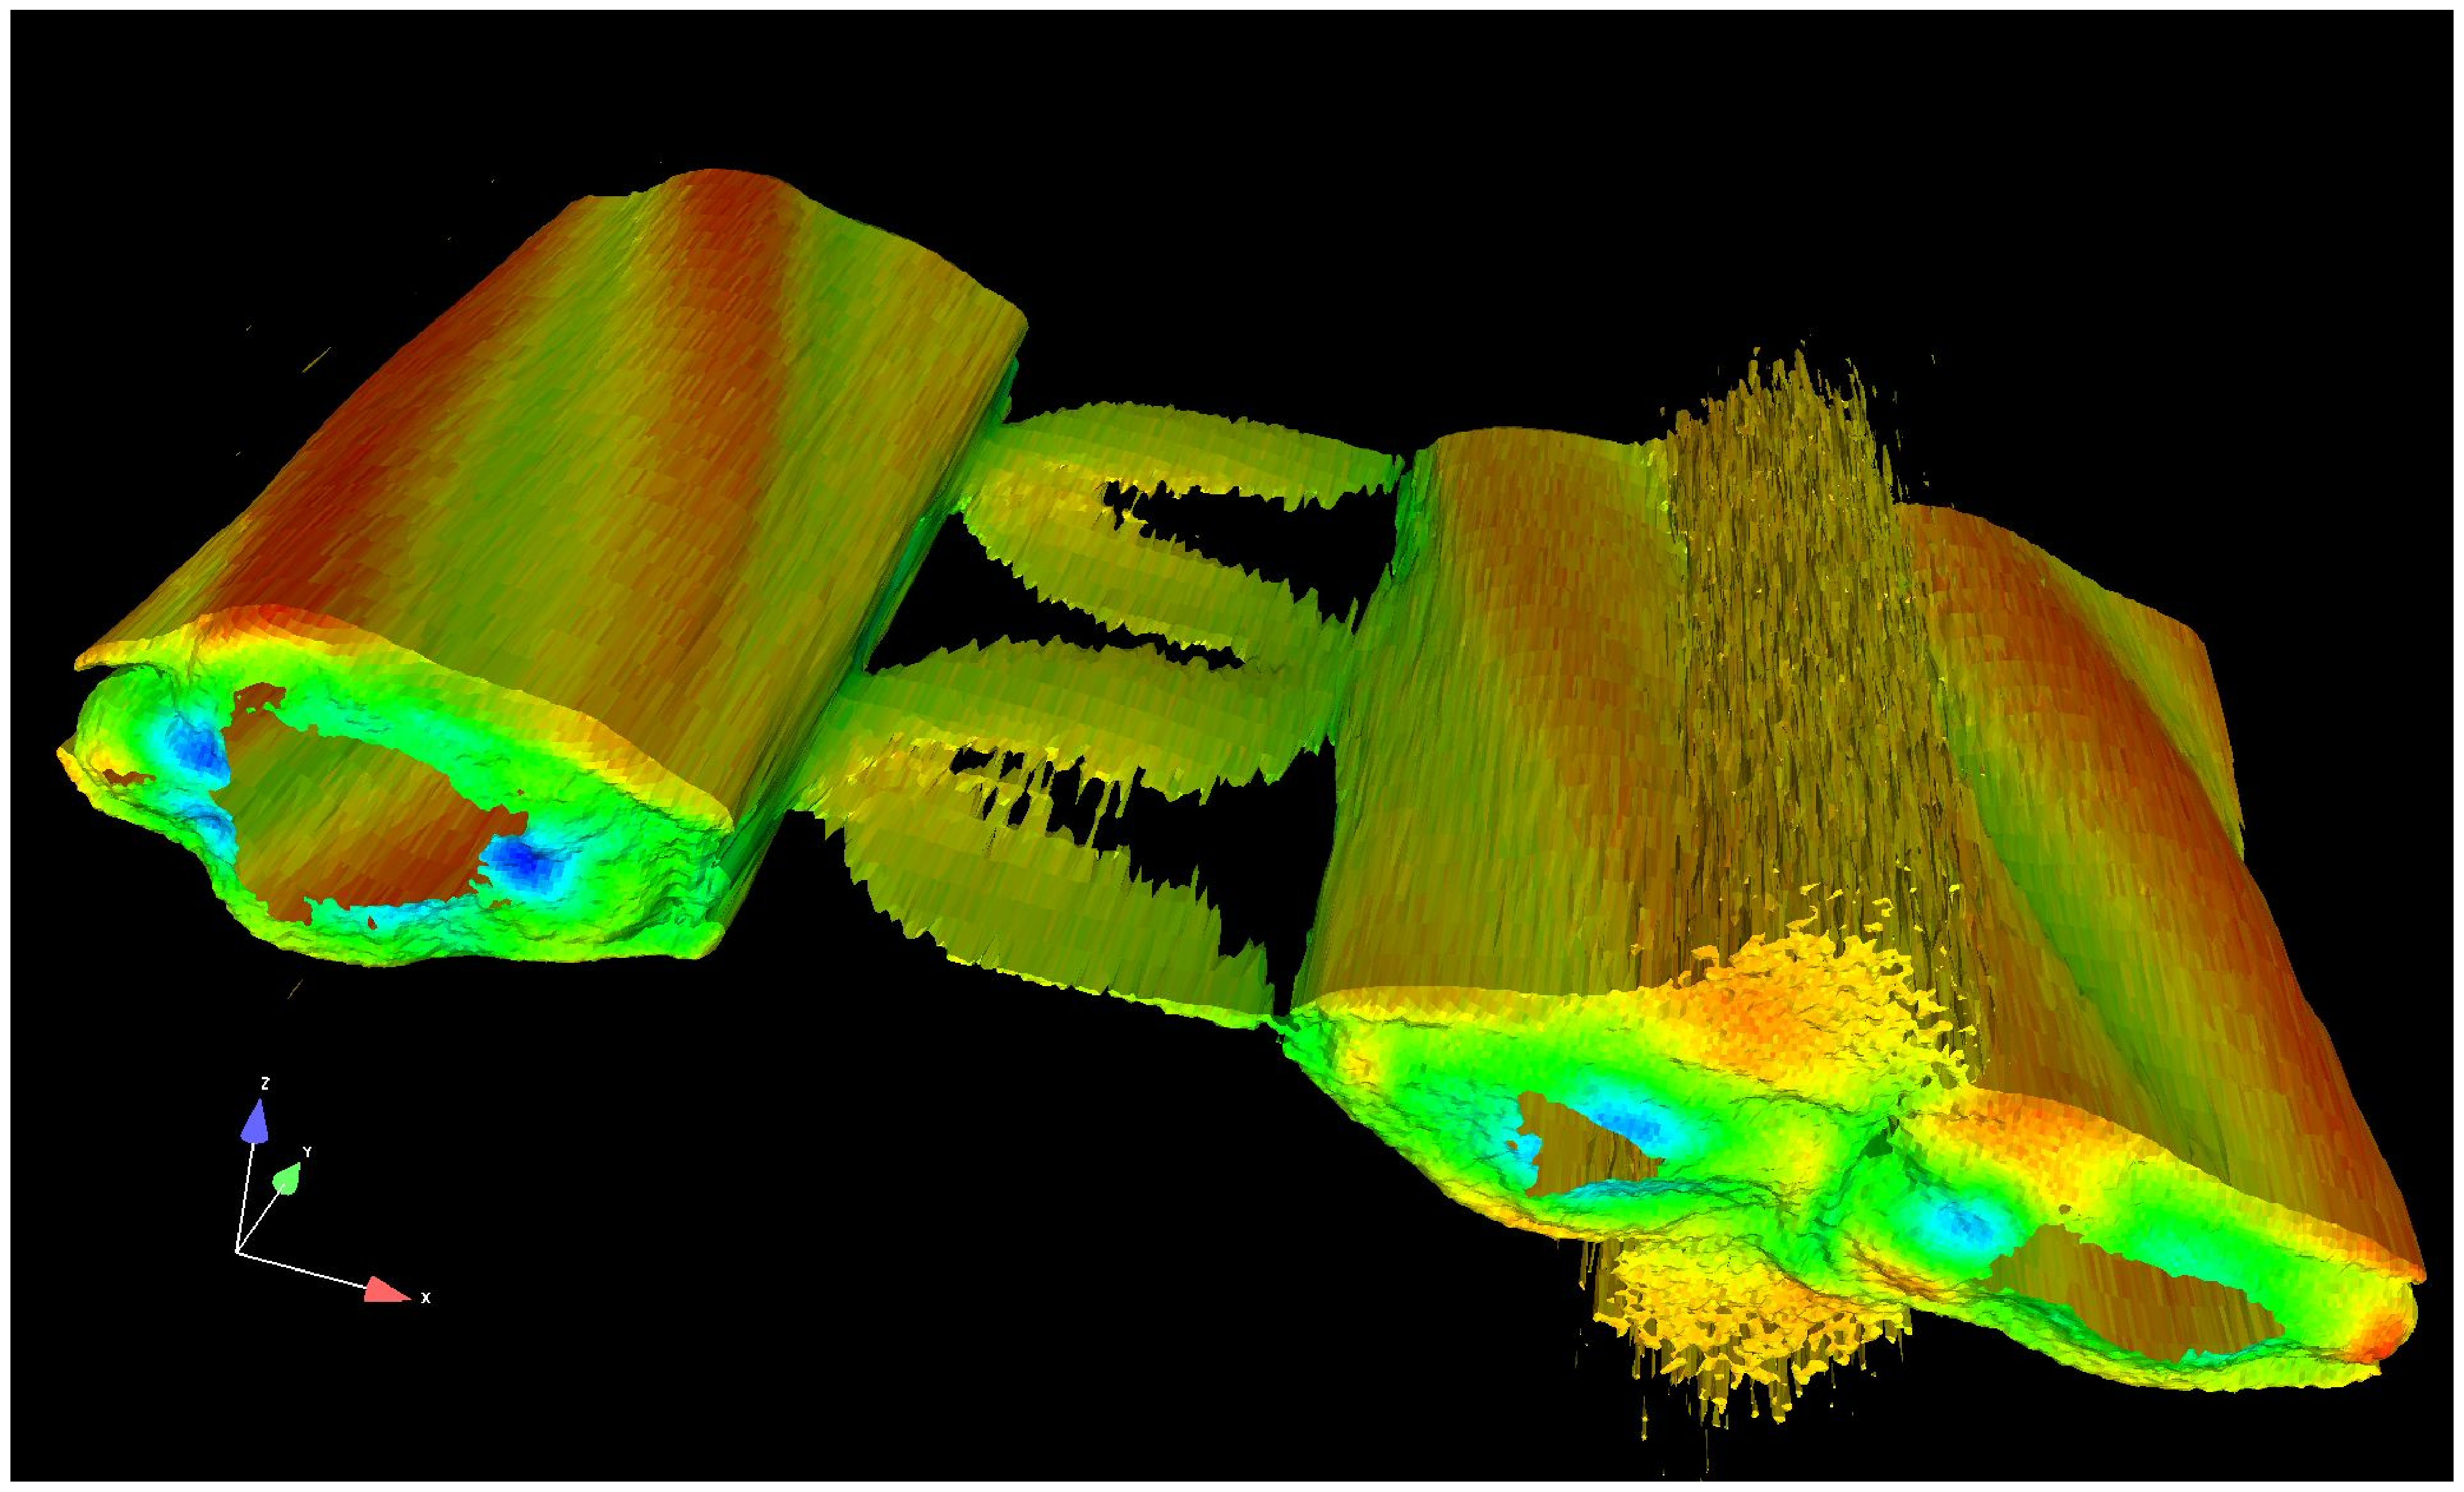
\includegraphics[width=75mm]{magnetic_reconnection.eps}
\caption{\label{fig:magnetic_reconnection}
(Color) 3D VPIC simulation of magnetic reconnection in a pair plasma
with an intermediate guide field.  Displayed are isosurfaces of
electron density colored by the magnetic field $B_y$ ($y$ is the
initial current and guide field direction).  The isosurfaces undulate
from the interaction of the tearing modes (wave vector along $x$) with
the drift-kink modes (along $y$). \cite{Yin_et_al_PRL_2007_reconnection}}
\end{figure}

VPIC has been applied with success in both basic and applied plasma
science.  Here, we give three examples of computationally demanding
simulations enabled by the high efficiency of VPIC.  The first is a
large-scale simulation of 3D magnetic reconnection in an
electron-positron plasma, as shown in \fig{magnetic_reconnection}.
The initial configuration is a Harris equilibrium with an intermediate
guide field.  The simulation follows the dynamics of 16 billion
particles on a $1000\times100\times1000$ mesh (on a physical domain of
$200d_i\times20d_i\times200d_i$ where $d_i$ is the ion inertial
length).  Shown are electron density isosurfaces with color indicating
the magnetic field $B_y$ ($y$ is the direction of initial current) at
a time when a dominant diffusion region has formed and influenced by
the drift-kink mode.  The calculation ran for 36 hours of wall-clock
time on 500 AMD Opteron cores. More details on the 3D reconnection
dynamics and the interplay between tearing and kink instability can be
found in \cite{Yin_et_al_PRL_2007_reconnection} (another examples of a
VPIC magnetic reconnection simulation is \cite{Bowers_Li_PRL_2007}).

\begin{figure}
\centering
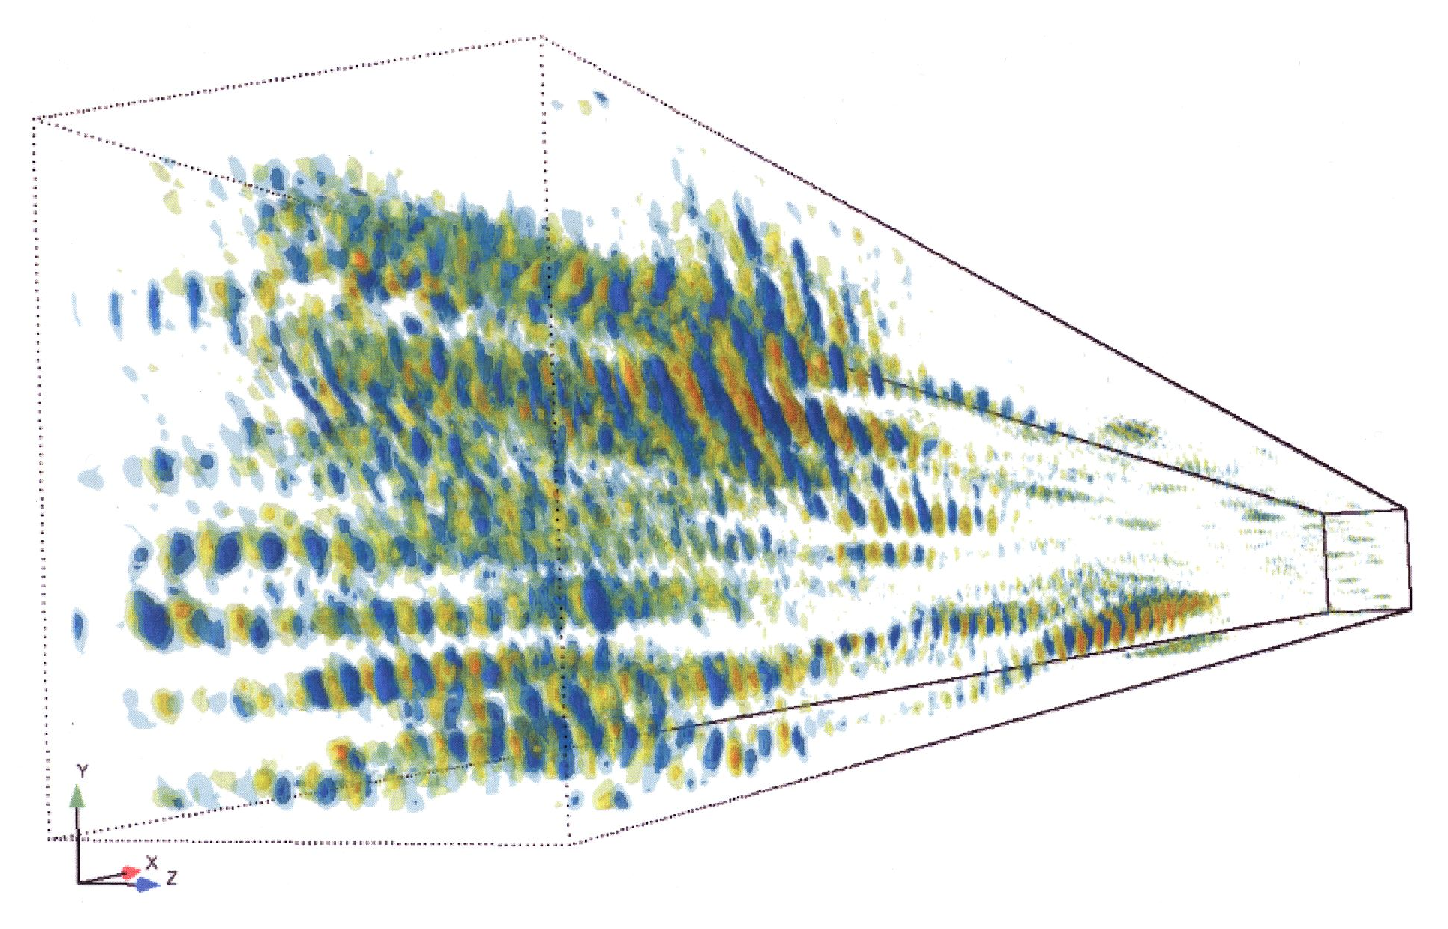
\includegraphics[width=75mm]{stimulated_raman_scattering.eps}
\caption{\label{fig:stimulated_raman_scattering}
(Color) 3D VPIC simulation of stimulated raman scattering (SRS) in the
kinetic regime.  Isosurfaces of longitudinal electrostatic field show
filament structures resulting from trapped electron self-focusing of
Langmuir waves during SRS saturation.  The laser is launched from the
simulation geometry near face.
\cite{Yin_et_al_Phys_Plasmas_2007_SRS}.}
\end{figure}

The second example in \fig{stimulated_raman_scattering} is a 3D
simulation of stimulated Raman scattering (SRS) in the kinetic regime
($k \lambda_d = 0.34$, where $k$ is the initial Langmuir wavenumber
and $\lambda_d$ is the plasma Debye length).  The simulation used 18
billion particles on a mesh of size $2436 \times 486 \times 486$ (on a
physical domain of $90\times18\times18$ microns) run on 1008 AMD
Opteron cores.  The electron plasma waves self-localize to regions of
narrow transverse extent, as shown by the filament structures in the
longitudinal electric field.  SRS saturates via the trapped electron
self-focusing of Langmuir waves
\cite{Yin_et_al_Phys_Plasmas_2007_SRS}.

\begin{figure}
\centering
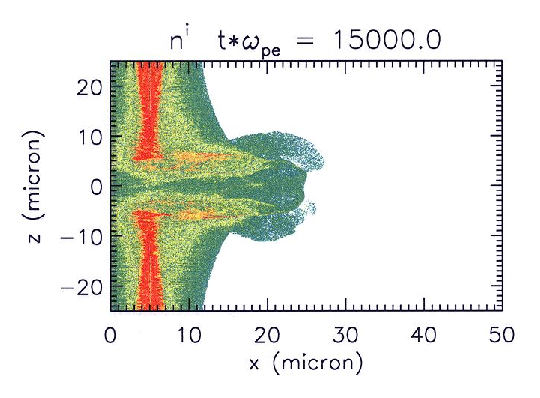
\includegraphics[width=83mm]{break_out_afterburner.eps}
\put(-90,60){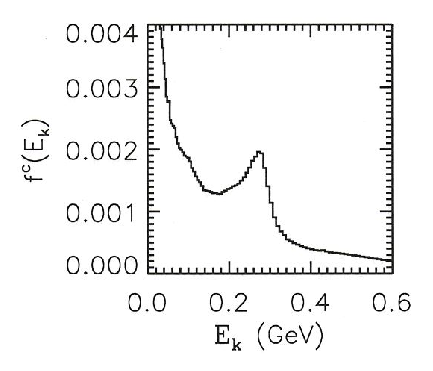
\includegraphics[width=27mm]{break_out_afterburner_inset.eps}}
\caption{\label{fig:break_out_afterburner}
(Color) Large-scale 2D VPIC simulation of ultra-intense laser
interaction with a thin target in the ``break-out afterburner''
regime.  Shown are contours of density for the carbon target as the
laser, launched from the simulation left edge, has propagated to the
simulation right edge; the inset displays the carbon energy spectrum,
obtained along a $1$~$\mu$m slice centered at $z=0$, with a
quasi-monoenergetic feature at $\sim 275$~MeV.
\cite{Yin_et_al_Phys_Plasmas_2007_BOA,Albright_et_al_Phys_Plasmas_2007}.}
\end{figure}

The final example shown in \fig{break_out_afterburner} is a
grid-dominated simulation of short-pulse laser interaction with a
solid density carbon target ($n_e/n_{\rm cr} = 660$, where $n_{\rm
cr}$ is the critical density).  This large-scale 2D simulation used
1.23 billion cells (on a physical domain of $50\times50$ microns) and
ran on 1020 AMD Opteron cores; within the ultrathin 30-nm-thick
target, each species is represented by $1.7\times10^5$ particles/cell.
Shown is the ion density after the $1$~$\mu$m laser, (a Gaussian beam
of FWHM 156~fs at an intensity of $10^{21}$~W/cm$^2$) launched from
the simulation left edge, has propagated to simulation right edge at
time 312~fs.  The inset displays the carbon energy spectrum with a
quasi-monoenergetic feature at $\sim 275$~MeV.  In the simulation,
quasi-monoenergetic and GeV carbon ions are generated via the
``Break-out Afterburner'' acceleration mechanism
\cite{Yin_et_al_Phys_Plasmas_2007_BOA,Albright_et_al_Phys_Plasmas_2007}.

\section{Conclusion}

If the LANL Roadrunner supercomputer is acquired as planned, VPIC
calculations will be possible in late 2008 at scales well beyond what
is practicable today: simulations with $10^{12}$ particles, $10^9$
cells, and $10^6$ time steps may be prosecuted in a matter of days.
This opens up the possibility for kinetic modeling of, e.g., 3D
magnetic reconnection at high ion-to-electron mass ratio for a
hydrogen plasma, 3D dynamics of stimulated laser scattering in
multi-speckles, 3D high resolution ultra-intense laser-matter
interaction, and \textit{ab initio} kinetic thermonuclear burn, to
name a few.  The techniques described herein that enable VPIC's
ultrahigh explicit PIC performance can be applied fruitfully to other
plasma simulation codes and platforms.  In this sense, VPIC is the
first of a new generation of high performance plasma simulation codes.

\begin{acknowledgments}
Work performed under the auspices of the United States Department of
Energy by the Los Alamos National Security LLC Los Alamos National
Laboratory under contract DE-AC52-06NA25396.  The authors acknowledge
the assistance of Drs. Hui Li and Bill Daughton.  3D visualization was
performed using the EnSight Gold software by CEI Inc.; the authors
thank Drs. Jeremy Margulies and Eric Nelson for their assistance.
Simulations shown were run on the LANL Flash and Lightning
supercomputers.
\end{acknowledgments}

\bibliography{paper}  

\end{document}
